
% ----------------------------------------------------------------------
%                   LATEX TEMPLATE FOR PhD THESIS
% ----------------------------------------------------------------------

% based on Harish Bhanderi's PhD/MPhil template, then Uni Cambridge
% http://www-h.eng.cam.ac.uk/help/tpl/textprocessing/ThesisStyle/
% corrected and extended in 2007 by Jakob Suckale, then MPI-CBG PhD programme
% and made available through OpenWetWare.org - the free biology wiki


%: Style file for Latex
% Most style definitions are in the external file PhDthesisPSnPDF.
% In this template package, it can be found in ./Latex/Classes/
\documentclass[twoside,11pt]{Latex/Classes/PhDthesisPSnPDF}


%: Macro file for Latex
% Macros help you summarise frequently repeated Latex commands.
% Here, they are placed in an external file /Latex/Macros/MacroFile1.tex
% An macro that you may use frequently is the figuremacro (see introduction.tex)
% This file contains macros that can be called up from connected TeX files
% It helps to summarise repeated code, e.g. figure insertion (see below).

% insert a centered figure with caption and description
% parameters 1:filename, 2:title, 3:description and label
\newcommand{\figuremacro}[3]{
	\begin{figure}[htbp]
		\centering
		\includegraphics[width=1\textwidth]{#1}
		\caption[#2]{\textbf{#2} - #3}
		\label{#1}
	\end{figure}
}

% insert a centered figure with caption and description AND WIDTH
% parameters 1:filename, 2:title, 3:description and label, 4: textwidth
% textwidth 1 means as text, 0.5 means half the width of the text
\newcommand{\figuremacroW}[4]{
	\begin{figure}[htbp]
		\centering
		\includegraphics[width=#4\textwidth]{#1}
		\caption[#2]{\textbf{#2} - #3}
		\label{#1}
	\end{figure}
}

% inserts a figure with wrapped around text; only suitable for NARROW figs
% o is for outside on a double paged document; others: l, r, i(inside)
% text and figure will each be half of the document width
% note: long captions often crash with adjacent content; take care
% in general: above 2 macro produce more reliable layout
\newcommand{\figuremacroN}[3]{
	\begin{wrapfigure}{o}{0.5\textwidth}
		\centering
		\includegraphics[width=0.48\textwidth]{#1}
		\caption[#2]{{\small\textbf{#2} - #3}}
		\label{#1}
	\end{wrapfigure}
}

% predefined commands by Harish
\newcommand{\PdfPsText}[2]{
  \ifpdf
     #1
  \else
     #2
  \fi
}

\newcommand{\IncludeGraphicsH}[3]{
  \PdfPsText{\includegraphics[height=#2]{#1}}{\includegraphics[bb = #3, height=#2]{#1}}
}

\newcommand{\IncludeGraphicsW}[3]{
  \PdfPsText{\includegraphics[width=#2]{#1}}{\includegraphics[bb = #3, width=#2]{#1}}
}

\newcommand{\InsertFig}[3]{
  \begin{figure}[!htbp]
    \begin{center}
      \leavevmode
      #1
      \caption{#2}
      \label{#3}
    \end{center}
  \end{figure}
}


%%% Local Variables: 
%%% mode: latex
%%% TeX-master: "~/Documents/LaTeX/CUEDThesisPSnPDF/thesis"
%%% End: 




%: ----------------------------------------------------------------------
%:                  TITLE PAGE: name, degree,..
% ----------------------------------------------------------------------
% below is to generate the title page with crest and author name

%if output to PDF then put the following in PDF header
\ifpdf  
    \pdfinfo { /Title  (Computer Aided Diagnosis system for prostatic biopsy guidance and follow-up fusing multi-modal imaging.
s)
               /Creator (TeX)
               /Producer (pdfTeX)
               /Author (Guillaume Lemaitre g.lemaitre58@gmail.com)
               /CreationDate (D:YYYYMMDDhhmmss)  %format D:YYYYMMDDhhmmss
               /ModDate (D:YYYYMMDDhhmm)
               /Subject (PhD Dissertation of Guillaume Lemaitre)
               /Keywords (CAD, prostatic biopsy, spectroscopy, MRI) }
    \pdfcatalog { /PageMode (/UseOutlines)
                  /OpenAction (fitbh)  }
\fi


\title{Computer Aided Diagnosis system for prostatic biopsy guidance and follow-up fusing multi-modal imaging.
}



% ----------------------------------------------------------------------
% The section below defines www links/email for author and institutions
% They will appear on the title page of the PDF and can be clicked
\ifpdf
  \author{\href{mailto:guillaume.lemaitre@udg.edu}{Guillaume Lema\^itre}}
%  \cityofbirth{born in XYZ} % uncomment this if your university requires this
%  % If city of birth is required, also uncomment 2 sections in PhDthesisPSnPDF
%  % Just search for the "city" and you'll find them.
  % The crest is a graphics file of the logo of your research institution.
  % Place it in ./0_frontmatter/figures and specify the width

%% First university
  \firstlab{\href{http://le2i.cnrs.fr/}{LE2I}}
  \firstlogolab{
\includegraphics[width=2cm]{logos/logole2i.eps}}
  \firstuni{\href{http://www.u-bourgogne.fr/}{Universit\'e de Bourgogne}}
  \firstlogouni{
\includegraphics[width=2cm]{logos/logo-ub-no-bg.pdf}}

  
%% Second university
  \secondlab{\href{http://vicorob.udg.es/}{ViCOROB}}
  \secondlogolab{
\includegraphics[width=2cm]{logos/vicorobLogo1.png}}

  \seconduni{\href{https://www.udg.edu/}{Universitat de Girona}}
  \secondlogouni{
\includegraphics[scale =0.5]{logos/UdG_dues_linies_centrat_blau.png}}
  
  \supervisora{Jordi Freixenet Bosch (ViCOROB - UdG)}
  \supervisorb{Fabrice M\'eriaudeau (CISIR - UTP)}
  \supervisorc{Robert Mar\'i Marly (ViCOROB - UdG)}
  \supervisord{Paul Michael Walker (LE2I - UBFC)}
  
% If you are not creating a PDF then use the following. The default is PDF.
\else
  \author{Guillaume Lema\^itre}
%  \cityofbirth{born in XYZ}
%% First university
  \firstlab{\href{http://le2i.cnrs.fr/}{LE2I}}
  \firstlogolab{
\includegraphics[width=2cm]{logos/logole2i.eps}}
  \firstuni{\href{http://www.u-bourgogne.fr/}{Universit\'e de Bourgogne}}
  \firstlogouni{
\includegraphics[width=2cm]{logos/logoubblue.eps}}
  
%% Second university
  \secondlab{\href{http://vicorob.udg.es/}{ViCOROB}}
  \secondlogolab{
\includegraphics[width=2cm]{logos/logovicorob.eps}}
  \seconduni{\href{https://www.udg.edu/}{Universitat de Girona}}
  \secondlogouni{
\includegraphics[width=2cm]{logos/logoudg.eps}}
  
  \supervisora{Jordi Freixenet Bosch (ViCOROB - UdG)}
  \supervisorb{Fabrice M\'eriaudeau (CISIR - UTP)}
  \supervisorc{Robert Mar\'i Marly (ViCOROB - UdG)}
  \supervisord{Paul Michael Walker (LE2I - UBFC)}
\fi

%\renewcommand{\submittedtext}{change the default text here if needed}
\degree{Philosophi\ae Doctor (PhD)}
\degreedate{April 2015}


% ----------------------------------------------------------------------
       
% turn of those nasty overfull and underfull hboxes
\hbadness=10000
\hfuzz=50pt


%: --------------------------------------------------------------
%:                  FRONT MATTER: dedications, abstract,..
% --------------------------------------------------------------

\begin{document}

%\language{english}

% sets line spacing
\renewcommand\baselinestretch{1.2}
\baselineskip=18pt plus1pt


%: ----------------------- generate cover page ------------------------

\maketitle  % command to print the title page with above variables


%: ----------------------- cover page back side ------------------------
% Your research institution may require reviewer names, etc.
% This cover back side is required by Dresden Med Fac; uncomment if needed.

\newpage
\vspace{10mm}
1. Reviewer: Name

\vspace{10mm}
2. Reviewer: 

\vspace{20mm}
Day of the defense:

\vspace{20mm}
\hspace{70mm}Signature from head of PhD committee:



%: ----------------------- abstract ------------------------

% Your institution may have specific regulations if you need an abstract and where it is to be placed in the document. The default here is just after title.


% Thesis Abstract -----------------------------------------------------


%\begin{abstractslong}    %uncommenting this line, gives a different abstract heading
\begin{abstracts}        %this creates the heading for the abstract page
Prostate cancer (CaP) is the second most diagnosed cancer in men all over the world.
CaP growth is characterized by two main types of evolution: (i) the slow-growing tumours progress slowly and usually remain confined to the prostate gland; (ii) the fast-growing tumours metastasize from prostate gland to other organs, which might lead to incurable diseases.
Therefore, early diagnosis and risk assessment play major roles in patient treatment and follow-up.
In the last decades, new imaging techniques based on Magnetic Resonance Imaging (MRI) have been developed improving diagnosis.
In practise, diagnosis can be affected by multiple factors such as observer variability and visibility and complexity of the lesions.
In this regard, computer-aided detection and computer-aided diagnosis systems are being designed to help radiologists in their clinical practice.

Our research extensively analyzes the current state-of-the-art in the development of computer-aided diagnosis and detection systems for prostate cancer detection.
Currently, no computer-aided system using all available MRI modalities has been proposed and tested on a common dataset.
Therefore, we propose a new computer-aided system taking advantage of all MRI modalities (i.e., \acs{t2w}-\acs{mri}, \acs{dce}-\acs{mri}, DW-\acs{mri}, \acs{mrsi}).
Particular attention is paid to the normalization of the \acs{mri} modalities prior to develop our computer-aided system.
This system has been extensively tested on a dataset which has been made publicly available.
\end{abstracts}
%\end{abstractlongs}
%-------------------------------------------------------------------------

\begin{abstractCatalan}

El c\`ancer de pr\`ostata (CaP) \'es el segon c\`ancer m\'es diagnosticat en homes a tot el m\'on.
El creixement del CaP es caracteritza per dos tipus principals d'evoluci\'o: (i) els tumors de creixement lent que progressen lentament i en general romanen confinats en la gl\`andula de la pr\`ostata; (Ii) els tumors de creixement r\`apid que desenvolupen met\`astasi de la pr\`ostata a altres \`organs, el que podria conduir a malalties incurables.
Conseqüentment, el diagn\`ostic preco\c{c} i l'avaluaci\'o del risc exerceixen un paper important en el tractament del pacient i el seguiment.
En les \'ultimes dècades s'han desenvolupat noves t\'ecniques d'imatge basades en imatge de resson\'ancia magn\`etica (RM, o MRI de l'angl\`es) per millorar el diagnòstic.
A la pr\`actica, el diagn\`ostic pot ser afectat per diversos factors com ara la variabilitat de l'observador i la visibilitat i la complexitat de les lesions.
En aquest sentit, s'estan desenvolupant sistemes per a l'ajuda a la detecci\'o i diagn\`ostic per ordinador per ajudar els radiòlegs en la seva pràctica clínica.

La nostra recerca analitza \`ampliament l'estat de l'art en el desenvolupament de sistemes per a l'ajuda a la detecci\'o i diagn\`ostic per ordinador per a la detecci\'o del c\`ancer de pr\`ostata.
En l'actualitat, no hi ha cap sistema d'ajuda al diagn\`ostic que utilitzi totes les modalitats de MRI disponibles i que hagi estat avaluat en un conjunt de dades com\'u.
Per tant, proposem un nou sistema d'ajuda al diagn\`ostic per ordinador aprofitant totes les modalitats de resson\`ancia magn\`etica (\'es a dir \acs{t2w}-MRI, DCE-MRI, DW-MRI, MRSI).
Com a etapa pr\`evia al desenvolupament del sistema, es presta especial atenci\'o a la normalitzaci\'o de les modalitats de resson\`ancia magn\`etica.
El sistema desenvolupat ha estat avaluat extensivament en un conjunt de dades que s'han posat a disposició pública.
 
\end{abstractCatalan}

% ---------------------------------------------------------------------- 
\begin{abstractSpanish}

El c\`ancer de pr\'ostata (CaP) es el segundo c\`ancer m\'as diagnosticado en hombres en todo el mundo.
El crecimiento del CaP se caracteriza por dos tipos principales de evoluci\'on: (i) los tumores de crecimiento lento que progresan lentamente y por lo general permanecen confinados en la gl\'andula de la pr\'ostata; (ii) los tumores de crecimiento r\'apido que desarrollan met\'astasis de la pr\'ostata a otros \'organos, lo que podr\'ia conducir a enfermedades incurables.
Consecuentemente, el diagn\'ostico precoz y la evaluaci\'on del riesgo desempe\~nan un papel importante en el tratamiento del paciente y el seguimiento. En las \'ultimas d\'ecadas se han desarrollado  nuevas t\'ecnicas de imagen basadas en imagen de resonancia magn\'etica (RM, o MRI del ingl\'es) para mejorar el diagn\'ostico. En la pr\'actica, el diagn\'ostico puede ser afectado por varios factores tales como la variabilidad del observador y la visibilidad y la complejidad de las lesiones.
En este sentido, se est\'an desarrollando sistemas para la ayuda a la detecci\'on y diagnóstico por ordenador para ayudar a los radi\'ologos en su pr\'actica cl\'inica.

Nuestra investigaci\'on analiza ampliamente el estado del arte en el desarrollo de sistemas para la ayuda a la detecci\'on y diagn\'ostico por ordenador para la detecci\'on del c\`ancer de pr\'ostata.
En la actualidad, no existe ning\'un sistema de ayuda al diagn\'ostico que utilice todas las modalidades de MRI disponibles y que haya sido evaluado en un conjunto de datos com\'un.
Por lo tanto, proponemos un nuevo sistema de ayuda al diagn\'ostico por ordenador aprovechando todas las modalidades de resonancia magnética (es decir T2W-MRI, DCE-MRI, DW-MRI, MRSI).
Como etapa previa al desarrollo del sistema, se presta especial atenci\'on a la normalizaci\'on de las modalidades de resonancia magn\'etica.
El sistema desarrollado ha sido evaluado extensivamente en un conjunto de datos que se han puesto a disposici\'on p\'ublica.
 
\end{abstractSpanish}

%-------------------------------------------------------------------------
\begin{abstractFrench}

Le cancer de la prostate est le second type de cancer le plus diagnostiqu\'e au monde.
Il est caract\'eris\'e par deux evolutions distinctes : (i) les tumeurs \`a croissances lentes progressent lentement et restent g\'en\'eralement confin\'ees dans la glande prostatique; (ii) les tumeurs \`a croissances rapides se m\'etastasent de la prostate \`a d'autres organes p\'eriph\'eriques, pouvant causer le d\'evelopement de maladies incurables.
C'est pour cela qu'un diagnostic pr\'ecoce et une \'evaluation du risque jouent des r\^oles majeurs dans le traitement et le suivi du patient.
Durant la derni\`ere d\'ec\'enie, de nouvelles m\'ethodes d'imagerie bas\'ees sur l'Imagerie par R\'esonance Magn\'etique (IRM) ont \'et\'e d\'evelop\'ees.
En pratique, le diagnostic clinique peut \^etre affect\'e par de multiples facteurs comme la variabilit\'e entre observateurs et la complexit\'e des l\'esions lues.
Pour ce faire, des syst\`emes de d\'etection et de diagnostic assist\'e par ordinateur (DAO) ont \'et\'e d\'evelop\'es pour aider les radiologistes durant leurs t\^aches cliniques.

Notre recherche analyse extensivement l'\'etat de l'art actuel concernant le d\'evelopement des syst\`emes de DAO pour la d\'etection du cancer de la prostate.
Actuellement, il n'\'existe aucun syst\`eme de DAO utilisant toutes les modalit\'es IRM disponibles et qui plus est, test\'e sur une base de donn\'ees commune.
Par cons\'equent, nous proposons un nouveau syst\`eme de DAO tirant profit de toutes les modalit\'es IRM (i.e., T2W-MRI, DCE-MRI, DW-MRI, MRSI).
Une attention particuli\`ere est port\'ee sur la normalisation de ces donn\'ees multi-param\'etriques avant la conception du syst\`eme de DAO.
De plus, notre syst\`eme de DAO a \'et\'e test\'e sur une base de donn\'ees que nous rendons publique.

\end{abstractFrench}


% The original template provides and abstractseparate environment, if your institution requires them to be separate. I think it's easier to print the abstract from the complete thesis by restricting printing to the relevant page.
%\begin{abstractseparate}
%  
% Thesis Abstract -----------------------------------------------------


%\begin{abstractslong}    %uncommenting this line, gives a different abstract heading
\begin{abstracts}        %this creates the heading for the abstract page
Prostate cancer (CaP) is the second most diagnosed cancer in men all over the world.
CaP growth is characterized by two main types of evolution: (i) the slow-growing tumours progress slowly and usually remain confined to the prostate gland; (ii) the fast-growing tumours metastasize from prostate gland to other organs, which might lead to incurable diseases.
Therefore, early diagnosis and risk assessment play major roles in patient treatment and follow-up.
In the last decades, new imaging techniques based on Magnetic Resonance Imaging (MRI) have been developed improving diagnosis.
In practise, diagnosis can be affected by multiple factors such as observer variability and visibility and complexity of the lesions.
In this regard, computer-aided detection and computer-aided diagnosis systems are being designed to help radiologists in their clinical practice.

Our research extensively analyzes the current state-of-the-art in the development of computer-aided diagnosis and detection systems for prostate cancer detection.
Currently, no computer-aided system using all available MRI modalities has been proposed and tested on a common dataset.
Therefore, we propose a new computer-aided system taking advantage of all MRI modalities (i.e., \acs{t2w}-\acs{mri}, \acs{dce}-\acs{mri}, DW-\acs{mri}, \acs{mrsi}).
Particular attention is paid to the normalization of the \acs{mri} modalities prior to develop our computer-aided system.
This system has been extensively tested on a dataset which has been made publicly available.
\end{abstracts}
%\end{abstractlongs}
%-------------------------------------------------------------------------

\begin{abstractCatalan}

El c\`ancer de pr\`ostata (CaP) \'es el segon c\`ancer m\'es diagnosticat en homes a tot el m\'on.
El creixement del CaP es caracteritza per dos tipus principals d'evoluci\'o: (i) els tumors de creixement lent que progressen lentament i en general romanen confinats en la gl\`andula de la pr\`ostata; (Ii) els tumors de creixement r\`apid que desenvolupen met\`astasi de la pr\`ostata a altres \`organs, el que podria conduir a malalties incurables.
Conseqüentment, el diagn\`ostic preco\c{c} i l'avaluaci\'o del risc exerceixen un paper important en el tractament del pacient i el seguiment.
En les \'ultimes dècades s'han desenvolupat noves t\'ecniques d'imatge basades en imatge de resson\'ancia magn\`etica (RM, o MRI de l'angl\`es) per millorar el diagnòstic.
A la pr\`actica, el diagn\`ostic pot ser afectat per diversos factors com ara la variabilitat de l'observador i la visibilitat i la complexitat de les lesions.
En aquest sentit, s'estan desenvolupant sistemes per a l'ajuda a la detecci\'o i diagn\`ostic per ordinador per ajudar els radiòlegs en la seva pràctica clínica.

La nostra recerca analitza \`ampliament l'estat de l'art en el desenvolupament de sistemes per a l'ajuda a la detecci\'o i diagn\`ostic per ordinador per a la detecci\'o del c\`ancer de pr\`ostata.
En l'actualitat, no hi ha cap sistema d'ajuda al diagn\`ostic que utilitzi totes les modalitats de MRI disponibles i que hagi estat avaluat en un conjunt de dades com\'u.
Per tant, proposem un nou sistema d'ajuda al diagn\`ostic per ordinador aprofitant totes les modalitats de resson\`ancia magn\`etica (\'es a dir \acs{t2w}-MRI, DCE-MRI, DW-MRI, MRSI).
Com a etapa pr\`evia al desenvolupament del sistema, es presta especial atenci\'o a la normalitzaci\'o de les modalitats de resson\`ancia magn\`etica.
El sistema desenvolupat ha estat avaluat extensivament en un conjunt de dades que s'han posat a disposició pública.
 
\end{abstractCatalan}

% ---------------------------------------------------------------------- 
\begin{abstractSpanish}

El c\`ancer de pr\'ostata (CaP) es el segundo c\`ancer m\'as diagnosticado en hombres en todo el mundo.
El crecimiento del CaP se caracteriza por dos tipos principales de evoluci\'on: (i) los tumores de crecimiento lento que progresan lentamente y por lo general permanecen confinados en la gl\'andula de la pr\'ostata; (ii) los tumores de crecimiento r\'apido que desarrollan met\'astasis de la pr\'ostata a otros \'organos, lo que podr\'ia conducir a enfermedades incurables.
Consecuentemente, el diagn\'ostico precoz y la evaluaci\'on del riesgo desempe\~nan un papel importante en el tratamiento del paciente y el seguimiento. En las \'ultimas d\'ecadas se han desarrollado  nuevas t\'ecnicas de imagen basadas en imagen de resonancia magn\'etica (RM, o MRI del ingl\'es) para mejorar el diagn\'ostico. En la pr\'actica, el diagn\'ostico puede ser afectado por varios factores tales como la variabilidad del observador y la visibilidad y la complejidad de las lesiones.
En este sentido, se est\'an desarrollando sistemas para la ayuda a la detecci\'on y diagnóstico por ordenador para ayudar a los radi\'ologos en su pr\'actica cl\'inica.

Nuestra investigaci\'on analiza ampliamente el estado del arte en el desarrollo de sistemas para la ayuda a la detecci\'on y diagn\'ostico por ordenador para la detecci\'on del c\`ancer de pr\'ostata.
En la actualidad, no existe ning\'un sistema de ayuda al diagn\'ostico que utilice todas las modalidades de MRI disponibles y que haya sido evaluado en un conjunto de datos com\'un.
Por lo tanto, proponemos un nuevo sistema de ayuda al diagn\'ostico por ordenador aprovechando todas las modalidades de resonancia magnética (es decir T2W-MRI, DCE-MRI, DW-MRI, MRSI).
Como etapa previa al desarrollo del sistema, se presta especial atenci\'on a la normalizaci\'on de las modalidades de resonancia magn\'etica.
El sistema desarrollado ha sido evaluado extensivamente en un conjunto de datos que se han puesto a disposici\'on p\'ublica.
 
\end{abstractSpanish}

%-------------------------------------------------------------------------
\begin{abstractFrench}

Le cancer de la prostate est le second type de cancer le plus diagnostiqu\'e au monde.
Il est caract\'eris\'e par deux evolutions distinctes : (i) les tumeurs \`a croissances lentes progressent lentement et restent g\'en\'eralement confin\'ees dans la glande prostatique; (ii) les tumeurs \`a croissances rapides se m\'etastasent de la prostate \`a d'autres organes p\'eriph\'eriques, pouvant causer le d\'evelopement de maladies incurables.
C'est pour cela qu'un diagnostic pr\'ecoce et une \'evaluation du risque jouent des r\^oles majeurs dans le traitement et le suivi du patient.
Durant la derni\`ere d\'ec\'enie, de nouvelles m\'ethodes d'imagerie bas\'ees sur l'Imagerie par R\'esonance Magn\'etique (IRM) ont \'et\'e d\'evelop\'ees.
En pratique, le diagnostic clinique peut \^etre affect\'e par de multiples facteurs comme la variabilit\'e entre observateurs et la complexit\'e des l\'esions lues.
Pour ce faire, des syst\`emes de d\'etection et de diagnostic assist\'e par ordinateur (DAO) ont \'et\'e d\'evelop\'es pour aider les radiologistes durant leurs t\^aches cliniques.

Notre recherche analyse extensivement l'\'etat de l'art actuel concernant le d\'evelopement des syst\`emes de DAO pour la d\'etection du cancer de la prostate.
Actuellement, il n'\'existe aucun syst\`eme de DAO utilisant toutes les modalit\'es IRM disponibles et qui plus est, test\'e sur une base de donn\'ees commune.
Par cons\'equent, nous proposons un nouveau syst\`eme de DAO tirant profit de toutes les modalit\'es IRM (i.e., T2W-MRI, DCE-MRI, DW-MRI, MRSI).
Une attention particuli\`ere est port\'ee sur la normalisation de ces donn\'ees multi-param\'etriques avant la conception du syst\`eme de DAO.
De plus, notre syst\`eme de DAO a \'et\'e test\'e sur une base de donn\'ees que nous rendons publique.

\end{abstractFrench}

%\end{abstractseparate}


%: ----------------------- tie in front matter ------------------------

\frontmatter
% Thesis Dedictation ---------------------------------------------------

\begin{dedication} %this creates the heading for the dedication page
\begin{flushright}
\textit{To my parents,\\
  to my brother and his family,\\
  to my wife,\\
  to those who are dear to my heart,\\
  and all those who find themselves in this work.}
\end{flushright}
\end{dedication}

% ----------------------------------------------------------------------

% Thesis Acknowledgements ------------------------------------------------


%\begin{acknowledgementslong} %uncommenting this line, gives a different acknowledgements heading
\begin{acknowledgements}      %this creates the heading for the acknowlegments
First and foremost, I would like to thank my supervisors, Dr. Mart\'i, Dr. M\'eriaudeau, Dr. Freixenet, and Dr. Walker for their constant support and guidance through this thesis.
I enjoyed every minute of our scientific discussions, barbecue dinner and unfinished nightly frozen trails.  
Without you this work would not simply be possible. 
Thanks to D\'esir\'e Sidib\'e as well for sharing his valuable knowledge and ideas. 

Thanks Cedric Demonceux, Olivier Morel, Josep Quintana for our trail and cycling breaks during the past years, Lets check the Strava two months after the defence.
And of course thanks to all my friends; Abir, Armine, Cansen, David, DP, Fran\c{c}ois, Amanda, Konstantine, Habib, Sarah, Sharad, Josep, Sergi, Mireia, Sonia, Shihav and last but not least Sik -for our endless scientific related discussion, ideas, excitements and disappointments.
Special thanks to Joseta, Aina, Montse, Mireia and Nathalie for their constant and patient help with my endless paperwork and questions.
I also would like to thank the reviewers, Dr. Su Ruan and Dr. Reyer Zwiggelaar and the other members of the panel for evaluating my work.

Last but not least, I would like to thank my family that has always being there fore me with their endless love and support, my parents, Ginnette and Patrice, brother, cedric and his family, Vero, Julian and Sarah. 
I would like to thank the family of my wife, although being far away I apprecaite your concerns and supports. 

Finally I would like to thank my wife, mojdeh ..... . 

   

\end{acknowledgements}
%\end{acknowledgmentslong}

% ------------------------------------------------------------------------





%: ----------------------- contents ------------------------

\setcounter{secnumdepth}{3} % organisational level that receives a numbers
\setcounter{tocdepth}{3}    % print table of contents for level 3
\tableofcontents            % print the table of contents
% levels are: 0 - chapter, 1 - section, 2 - subsection, 3 - subsection


%: ----------------------- list of figures/tables ------------------------

\listoffigures	% print list of figures

\listoftables  % print list of tables


%: ----------------------- glossary ------------------------

% Tie in external source file for definitions: /0_frontmatter/glossary.tex
% Glossary entries can also be defined in the main text. See glossary.tex

% this file is called up by thesis.tex
% content in this file will be fed into the main document
\chapter*{Glossary}



\addcontentsline{toc}{chapter}{List of Abbreviations}

%\printacronyms[name = Abbreviations]
\printacronyms
 

%: --------------------------------------------------------------
%:                  MAIN DOCUMENT SECTION
% --------------------------------------------------------------

% the main text starts here with the introduction, 1st chapter,...
\mainmatter

%\renewcommand{\chaptername}{} % uncomment to print only "1" not "Chapter 1"


%: ----------------------- subdocuments ------------------------

% Parts of the thesis are included below. Rename the files as required.
% But take care that the paths match. You can also change the order of appearance by moving the include commands.


% this file is called up by thesis.tex
% content in this file will be fed into the main document

%: ----------------------- introduction file header -----------------------
\chapter{Introduction}

% the code below specifies where the figures are stored
\ifpdf
    \graphicspath{{1_introduction/figures/}}
\else
    \graphicspath{{1_introduction/figures/}}
\fi

%% ----------------------------------------------------------------------
%%: ----------------------- introduction content ----------------------- 
%% ----------------------------------------------------------------------
%
%
%
%%: ----------------------- HELP: latex document organisation
%% the commands below help you to subdivide and organise your thesis
%%    \chapter{}       = level 1, top level
%%    \section{}       = level 2
%%    \subsection{}    = level 3
%%    \subsubsection{} = level 4
%% note that everything after the percentage sign is hidden from output
%
%
%
%\section{put section name here} % section headings are printed smaller than chapter names
%% intro
%Write your text without any further commands, like this:.... Any organised system requires energy, be it a machine of some kind or a live organism. Energy is needed to win the uphill battle against entropy and pull together lifeless molecules to be able to do something in this world, like complete a PhD.
%
%
%
%\subsection{Name your subsection} % subsection headings are again smaller than section names
%% lead
%Different organised systems have different energy currencies. The machines that enable us to do science like sizzling electricity but at a controlled voltage. Earth's living beings are no different, except that they have developed another preference. They thrive on various chemicals. 
%
%% dextran, starch, glycogen
%Most organisms use polymers of glucose units for energy storage and differ only slightly in the way they link together monomers to sometimes gigantic macromolecules. Dextran of bacteria is made from long chains of $\alpha$-1,6-linked glucose units. 
%
%%: ----------------------- HELP: special characters
%% above you can see how special characters are coded; e.g. $\alpha$
%% below are the most frequently used codes:
%%$\alpha$  $\beta$  $\gamma$  $\delta$
%
%%$^{chars to be superscripted}$  OR $^x$ (for a single character)
%%$_{chars to be suberscripted}$  OR $_x$
%
%%>  $>$  greater,  <  $<$  less
%%≥  $\ge$  greater than or equal, ≤  $\ge$  lesser than or equal
%%~  $\sim$  similar to
%
%%$^{\circ}$C   ° as in degree C
%%±  \pm     plus/minus sign
%
%%$\AA$     produces  Å (Angstrom)
%
%
%
%
%% dextran, starch, glycogen continued
%Starch of plants and glycogen of animals consists of $\alpha$-1,4-glycosidic glucose polymers \cite{lastname07}. See figure \ref{largepotato} for a comparison of glucose polymer structure and chemistry. 
%
%Two references can be placed separated by a comma \cite{lastname07,name06}.
%
%%: ----------------------- HELP: references
%% References can be links to figures, tables, sections, or references.
%% For figures, tables, and text you define the target of the link with \label{XYZ}. Then you call cross-link with the command \ref{XYZ}, as above
%% Citations are bound in a very similar way with \cite{XYZ}. You store your references in a BibTex file with a programme like BibDesk.
%
%
%
%
%
%\figuremacro{largepotato}{A common glucose polymers}{The figure shows starch granules in potato cells, taken from \href{http://molecularexpressions.com/micro/gallery/burgersnfries/burgersnfries4.html}{Molecular Expressions}.}
%
%%: ----------------------- HELP: adding figures with macros
%% This template provides a very convenient way to add figures with minimal code.
%% \figuremacro{1}{2}{3}{4} calls up a series of commands formating your image.
%% 1 = name of the file without extension; PNG, JPEG is ok; GIF doesn't work
%% 2 = title of the figure AND the name of the label for cross-linking
%% 3 = caption text for the figure
%
%%: ----------------------- HELP: www links
%% You can also see above how, www links are placed
%% \href{http://www.something.net}{link text}
%
%\figuremacroW{largepotato}{Title}{Caption}{0.8}
%% variation of the above macro with a width setting
%% \figuremacroW{1}{2}{3}{4}
%% 1-3 as above
%% 4 = size relative to text width which is 1; use this to reduce figures
%
%
%
%
%Insulin stimulates the following processes:
%
%\begin{itemize}
%\item muscle and fat cells remove glucose from the blood,
%\item cells breakdown glucose via glycolysis and the citrate cycle, storing its energy in the form of ATP,
%\item liver and muscle store glucose as glycogen as a short-term energy reserve,
%\item adipose tissue stores glucose as fat for long-term energy reserve, and
%\item cells use glucose for protein synthesis.
%\end{itemize}
%
%%: ----------------------- HELP: lists
%% This is how you generate lists in LaTeX.
%% If you replace {itemize} by {enumerate} you get a numbered list.
%
%
% 
%
%
%%: ----------------------- HELP: tables
%% Directly coding tables in latex is tiresome. See below.
%% I would recommend using a converter macro that allows you to make the table in Excel and convert them into latex code which you can then paste into your doc.
%% This is the link: http://www.softpedia.com/get/Office-tools/Other-Office-Tools/Excel2Latex.shtml
%% It's a Excel template file containing a macro for the conversion.
%
%\begin{table}[htdp]
%\centering
%\begin{tabular}{ccc} % ccc means 3 columns, all centered; alternatives are l, r
%
%{\bf Gene} & {\bf GeneID} & {\bf Length} \\ 
%% & denotes the end of a cell/column, \\ changes to next table row
%\hline % draws a line under the column headers
%
%human latexin & 1234 & 14.9 kbps \\
%mouse latexin & 2345 & 10.1 kbps \\
%rat latexin   & 3456 & 9.6 kbps \\
%% Watch out. Every line must have 3 columns = 2x &. 
%% Otherwise you will get an error.
%
%\end{tabular}
%\caption[title of table]{\textbf{title of table} - Overview of latexin genes.}
%% You only need to write the title twice if you don't want it to appear in bold in the list of tables.
%\label{latexin_genes} % label for cross-links with \ref{latexin_genes}
%\end{table}
%
%
%
%% There you go. You already know the most important things.
%
%
%% ----------------------------------------------------------------------

% Prostate Cancer:
%%% This part contains:
%%% - Anatomy basis of the prostate
%%% - Statistics regarding prostate cancers
\section{Prostate Cancer}\label{section:intro:prostatecancer}

\subsection{Anatomy}\label{subsection:intro:prostatecancer:anatomy}

\begin{figure}
\centering
\includegraphics[height=0.25\textheight]{1_introduction/figures/anatomy/prostate2D.eps}
\caption{Sagittal anatomy scheme of the male reproductive system}
\label{fig:prostatelocation}
\end{figure}

\begin{figure}
	\centering
	\hspace*{\fill}
	\subfigure[Transverse anatomy of the prostate.]{
			\centering
			\includegraphics[height=0.15\textheight]{1_introduction/figures/anatomy/prostateTransverse.eps}
			\label{fig:anatomyProstateTransverse}}
			\hfill
	\subfigure[Sagittal anatomy of the prostate.]{
			\centering
			\includegraphics[height=0.23\textheight]{1_introduction/figures/anatomy/prostateSagital.eps}
			\label{fig:anatomyProstateSagittal}}\hspace*{\fill}
	\caption{Prostate anatomy with division in different zones. \textit{AFT:} anterior fibromuscular tissue, \textit{CZ:} central zone, \textit{ED:} ejaculatory duct, \textit{NVB:} neurovascular bundle, \textit{PUT:}  tissue, \textit{PZ:} peripheral zone, \textit{U:} urethra, \textit{TZ:} transitional zone, \textit{B:} base, \textit{M:} median, \textit{A:} apex (copyright by \cite{Choi2007}).}
	\label{fig:anatomyProstateZone}
\end{figure}

The prostate is an exocrine gland of the male reproductive system having an inverted pyramidal shape, which is located below the bladder and infront of the rectum (see Fig.~\ref{fig:prostatelocation}).
It measures approximately three centimetres in height by two and half centimetres in depth and its weight is estimated to be between seven and sixteen grams for an adult (\cite{Leissner1979}). The prostate size increases at two distinct stages during physical development: initially at puberty to reach its normal size, then again after sixty years of age leading to \ac{bph} (\cite{Parfait2010}).

A zonal classification of the prostate, depicted in \acs{fig} \ref{fig:anatomyProstateZone}, was suggested by McNeal (\cite{McNeal1981}). Subsequently, this categorization was widely accepted in the literature (cf., \cite{Hricak1987,Villers1991,Coakley2000,Parfait2010}) and is used in all medical examinations (e.g., biopsy, \ac{mri} screening). The classification is based on dividing the gland into three distinct regions: (i) \ac{cz} accounting for 20-25\% of the whole prostate gland, (ii) \ac{tz} standing for 5\% and (iii) \ac{pz} representing the 70\%. In \ac{mri} images, tissues of \ac{cz} and \ac{tz} are difficult to distinguish and are usually merged into a common region, denominated \ac{cg}.
As part of this classification, the prostate can be divided in three longitudinal portions depicted in \acs{fig} \ref{fig:anatomyProstateSagittal}: (i) base, (ii) median gland and (iii) apex.

%% \begin{figure}
%% 	\centering
%% 	\includegraphics[width=0.65\textwidth]{anatomy/prostate2D.eps}
%% 	\caption{Sagittal anatomy scheme of the male reproductive system \cite{Geckomedia2011}.}
%% 	\label{fig:intro:prostatecancer:anatomy:anatomyProstate2D}
%% \end{figure}


%% \begin{figure}
%% 	\centering
%% 	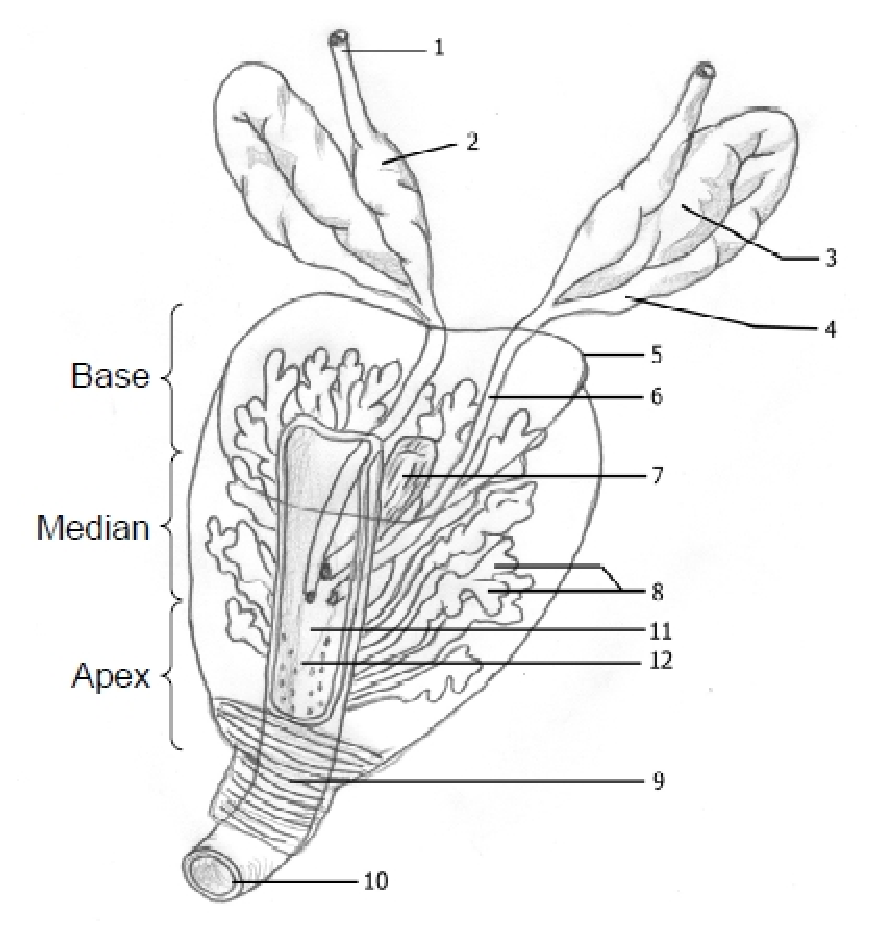
\includegraphics[width=0.50\textwidth]{anatomy/prostate2D2.eps}
%% 	\caption{Representation of the prostate. 1: Vas deferens, 2: Ampulla, 3: Seminal vesicle, 4: Excretory duct of seminal vesicle, 5: Prostate contour, 6: Ejaculatory duct, 7: Prostatic urticle, 8: Glandular tissue, 9: Urethral sphincter, 10: Urethra, 11: Seminal colliculus, 12: Urethral crest \cite{Wikipedia2011}.}
%% 	\label{fig:intro:prostatecancer:anatomy:anatomyProstate2D2}
%% \end{figure}


%% \begin{figure}
%% 	\centering
%% 	\subfigure[Transverse anatomy of the prostate.]{
%% 			\centering
%% 			\includegraphics[width=0.4\textwidth]{anatomy/prostateTransverse.eps}
%% 			\label{fig:anatomyProstateTransverse}}
%% 	~~~
%% 	\subfigure[Sagital anatomy of the prostate.]{
%% 			\centering
%% 			\includegraphics[width=0.4\textwidth]{anatomy/prostateSagital.eps}
%% 			\label{fig:anatomyProstateSagital}}
%% 	\caption{Presentation of the different zones of the prostate. \textit{AFT:} anterior fibromuscular tissue, \textit{CZ:} central zone, \textit{ED:} ejaculatory duct, \textit{NVB:} neurovascular bundle, \textit{PUT:} periurethral tissue, \textit{PZ:} peripherical zone, \textit{U:} urethra, \textit{TZ:} transitional zone \cite{Choi2007}.}
%% 	\label{fig:intro:prostatecancer:anatomy:anatomyProstateZone}
%% \end{figure}

\subsection{Prostate Carcinoma}
\ac{cap} has been reported on a worldwide scale to be the second most frequently diagnosed cancer of men accounting for $13.6 \%$ (\cite{Ferlay2010}). Statistically, in 2008, the number of new diagnosed cases was estimated to be $899,000$ with no less than $258,100$ deaths (\cite{Ferlay2010}). In United States, aside from skin cancer, \ac{cap} was declared to be the most commonly diagnosed cancer among men, implying that approximately one in six men will be diagnosed with \ac{cap} during their lifetime and one in thirty-six will die from this disease causing \ac{cap} to be the second most common cause of cancer death among men (\cite{Siegel2013}, \cite{Society2013}).

Despite active research to determine the causes of prostate cancer, a fuzzy list of risk factors has arisen (\cite{Society2010}). The etiology was linked to the following factors (\cite{Society2010}): (i) family history (\cite{Giovannucci2007,Steinberg1990}), (ii) genetic factors (\cite{Freedman2006,Amundadottir2006,Agalliu2009}), (iii) race-ethnicity (\cite{Giovannucci2007,Hoffman2001}), (iv) diet (\cite{Giovannucci2007,Ma2009,Alexander2010}), (v) obesity (\cite{Giovannucci2007,Rodriguez2007}). This list of risk factors alone cannot be used to diagnose CaP and in this way, screening enables early detection and treatment.

\ac{cap} growth is characterized by two main types of evolution (\cite{Strum2005}): slow-growing tumours, accounting for up to 85 \% of all \acp{cap} (\cite{Lu-Yao2009}), progress slowly and usually stay confined to the prostate gland. For such cases, treatment can be substituted with active surveillance. In contrast, the second variant of \acp{cap} develops rapidly and metastasises from prostate gland to others organs, primarily the bones (\cite{Oster2013}). Bone metastases, being an incurable disease, significantly affects the morbidity and mortality rate (\cite{Ye2007}). Hence, the  results of the surveillance have to be trustworthy in order to distinguish aggressive from slow-growing \ac{cap}.

\ac{cap} is more likely to come into being in specific regions of the prostate. In that respect, around 70-80 \% of \acp{cap} originate in \ac{pz} whereas 10-20 \% in \ac{tz} (\cite{Carrol1987,McNeal1988,Stamey1998}). Only about 5 \% of \acp{cap} occur in \ac{cz} (\cite{McNeal1988,Cohen2008}). However, those cancers appear to be more aggressive and more likely to invade other organs due to their location (\cite{Cohen2008}).


\subsection{Statistics}\label{subsection:intro:prostatecancer:statistics}

\subsubsection{Overview}\label{subsubsection:intro:prostatecancer:statistics:overview}

The World Health Organization (WHO) published in 2008 that PCa was the second most frequently diagnosed cancer of men and the fifth most common cancer overall \cite{Ferlay2010}. No less than 899,000 new cases where detected worldwide in 2008 \cite{Ferlay2010}. As presented on Fig. \ref{fig:intro:prostatecancer:statistics:overview:repartitionCancer}, PCa accounts for approximately 7.1\% (Fig. \ref{fig:intro:prostatecancer:statistics:overview:repartitionCancerIncidence}) of all cancers diagnosed in 2008 and 3.4\% (Fig. \ref{fig:intro:prostatecancer:statistics:overview:repartitionCancerDeaths}) of all cancers deaths in 2008 \cite{Ferlay2010}.

\begin{figure}
	\centering
	\subfigure[Estimated number cancers cases for both sexes and all ages.]{
			\centering
			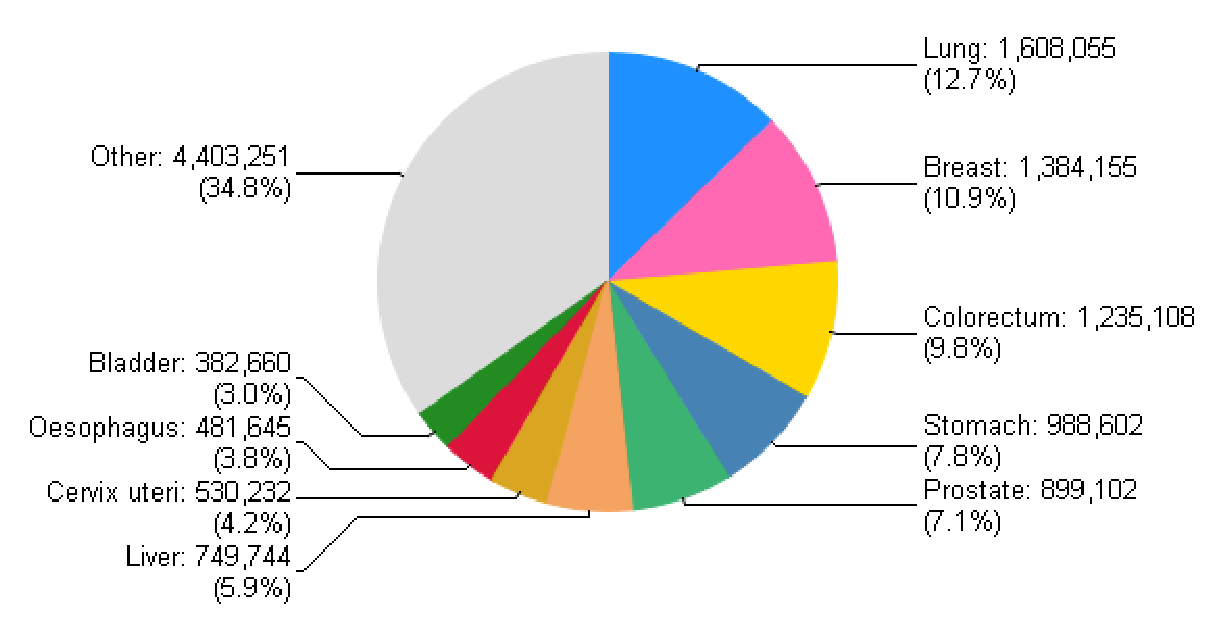
\includegraphics[width=0.65\textwidth]{statistics/repartitionCancerIncidence.eps}
			\label{fig:intro:prostatecancer:statistics:overview:repartitionCancerIncidence}}
	~
	\subfigure[Estimated number cancers deaths for both sexes and all ages.]{
			\centering
			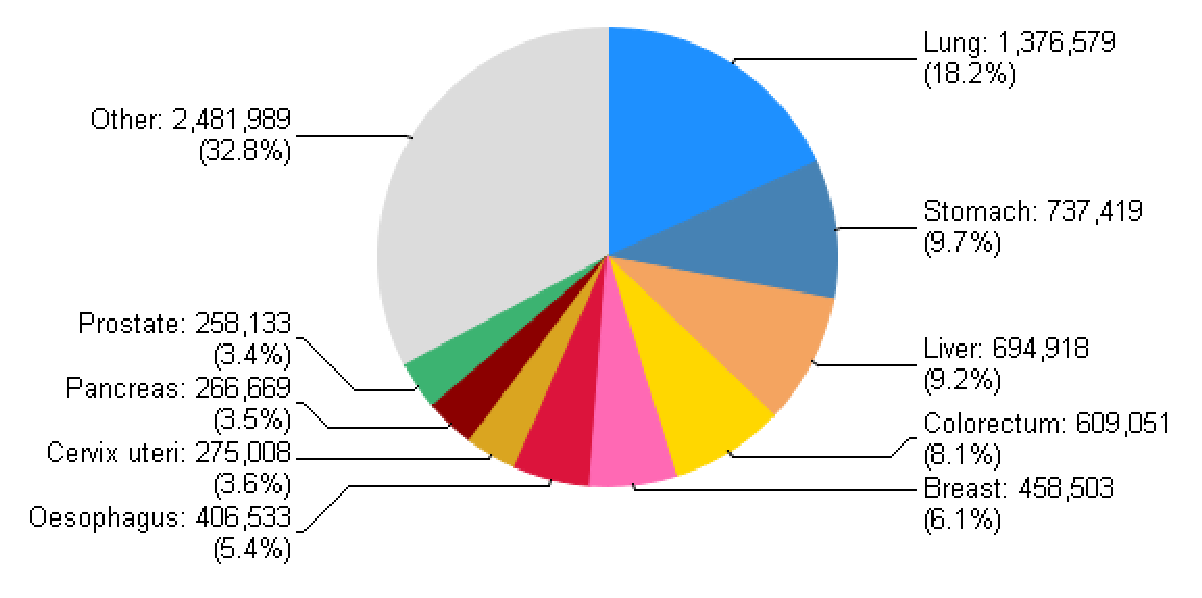
\includegraphics[width=0.65\textwidth]{statistics/repartitionCancerDeaths.eps}
			\label{fig:intro:prostatecancer:statistics:overview:repartitionCancerDeaths}}
	\caption{Cancer estimations in 2008 by the World Health Organization (WHO) \cite{Ferlay2010}.}
	\label{fig:intro:prostatecancer:statistics:overview:repartitionCancer}
\end{figure}

\subsubsection{Risk Factors}\label{subsubsection:intro:prostatecancer:statistics:riskfactors}

The risk factors can be categorized in three different classes: 

\begin{itemize}
	\item Age: age is the most important risk factor for PCa. The diagnosis of PCa for men over 50 years old. PCa rate increases upto about 70 and declines thereafter \cite{AmericanCancerSociety2010}.
	\item Genetic factors: it has been shown that the probability to have a cancer is higher when a member of the family has been already diagnosed \cite{AmericanCancerSociety2010}.
	\item Race: in the United States, the Africo Americans have a higher probability of developing a PCa than European American and Hispanic men \cite{AmericanCancerSociety2010}.
\end{itemize}

%%%%%%%%%%%%%%%%%%%%%%%%%% From previous draft %%%%%%%%%%%%%%%%%%%%%%%%%%%%%%%%%%%%%%%%%%%%%%%%
%% \subsection{Diagnosis and Medical Exams}\label{subsubsection:intro:prostatecancer:diagnosis}

%% The presence of PCa may be suggested in several ways: digital rectal examination, Prostate Specific Antigen (PSA\g) test, biopsy using transrectal ultrasound (TRUS\g) and magnetic resonance imaging (MRI\g-MRSI\g).

%% \subsubsection{Digital Rectal Examination}\label{subsubsection:intro:prostatecancer:diagnosis:rectalexamination}
%% Both benign prostatic hyperplasia and cancer may lead to an increasing size of the prostate. A rectal examination may allow detection of harder nodules within the softer prostatic tissue. The advantages are that this method is very fast and does not need any special equipment.
%% \subsubsection{PSA test}\label{subsubsection:intro:prostatecancer:diagnosis:psa}
%% The PSA is a protein secreted by the prostate. A higher-than-normal level of PSA can indicate an abnormality of the prostate: a benign prostatic hyperplasia or a cancer. However, other factors can lead to an increasing level of PSA such as prostate infections, irritations, a recent ejaculation or a recent rectal examination, etc.
%% The PSA can be found in the blood in two different forms: free PSA (about 10\%) and linked to another protein (about 90\%).
%% A level of PSA higher than 10 $ng.mL^{-1}$ is considered as pathologic \cite{Parfait2010}. If the PSA level is between 10 $ng.mL^{-1}$ and 4 $ng.mL^{-1}$, the patient is considered as suspicious \cite{Parfait2010}. In that case, the ratio free PSA over total PSA is computed. If the ratio is higher than 15\%, the case is considered as pathologic.
%% \subsubsection{TRUS}\label{subsubsection:intro:prostatecancer:diagnosis:trus}
%% As described in Sect. \ref{subsection:intro:prostatecancer:anatomy}, the prostate is localized in front of the rectum. Hence, its position allows one to carry out a biopsy using transrectal ultrasound (TRUS) in order to localise more precisely an eventual cancer (Fig. \ref{fig:intro:prostatecancer:diagnosis:trus}).
%% \textbf{\textit{\textsc{Add example of images of TRUS PCa and not}}}
%% \begin{figure}
%% 	\centering
%% 	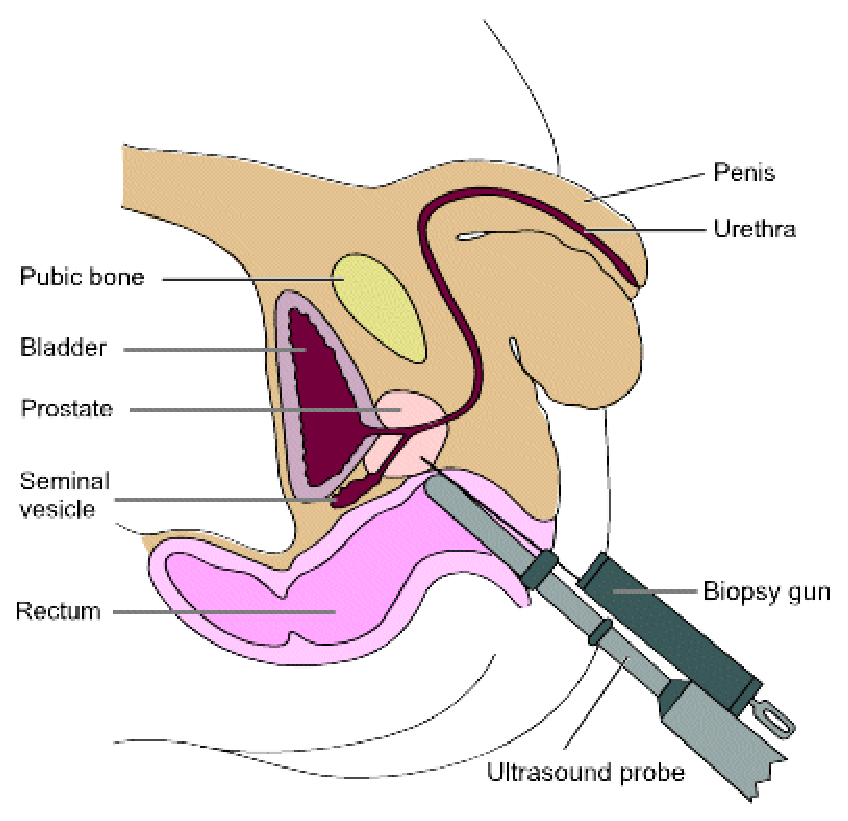
\includegraphics[width=0.45\textwidth]{diagnosis/trus/trus.eps}
%% 	\caption{Biopsy of the prostate using TRUS}
%% 	\label{fig:intro:prostatecancer:diagnosis:trus}
%% \end{figure}
%% \textbf{\textit{\textsc{Add information about protocol: manipulation of the patients, which equipment (see Jhimli thesis)}}}
%% The biopsy is usually prescribed when the PSA level is higher-than-normal or abnormalities were detected during a rectal examination. At least six different samples are taken from the right and left parts of the three different zones: apex, median and base. The samples are analysed in order to determine the presence of a cancer.
%% \textbf{\textit{\textsc{Add more information on the specificities and accuracy of the techniques. Add also what are the advantages (real-time)}}}

% MRI Principles:
%%% This part contains:
\section{Magnetic Resonance Imaging Principles}\label{section:intro:mriprinciples}



	% background information
% this file is called up by thesis.tex
% content in this file will be fed into the main document

\chapter{Aims of the project} % top level followed by section, subsection


% ----------------------- contents from here ------------------------

\section{Final aim}

Our ultimate goal is...

\section{Preliminary aims}

There will be several preliminary scientific targets to be accomplished on the way...




% ---------------------------------------------------------------------------
% ----------------------- end of thesis sub-document ------------------------
% ---------------------------------------------------------------------------						% aims of the project

% this file is called up by thesis.tex
% content in this file will be fed into the main document

\chapter{State of the art in multi-modal magnetic resonance imaging} % top level followed by section, subsection


% ----------------------- contents from here ------------------------

\section{Magnetic resonance imaging techniques}\label{section:stateart:mritechniques}

\subsection{Anatomic T2-weighted magnetic resonance imaging}\label{subsection:stateart:t2}

\subsubsection{Imaging characteristics}

As previously mentioned in Sect. \ref{subsubsection:intro:prostatecancer:diagnosis:mri}, T2-weighted MRI modality allows to clearly differentiate the prostate anatomy \cite{Hricak1987, Hoeks2011}. Indeed, high-intensity-signal of PZ is highly contrasted with low-signal-intensity of CZ or TZ \cite{Hoeks2011} (see Fig.\textbf{Add figure healthy T2}), while PCa is usually characterized by a very low-signal-intensity (\textbf{Add figure PCa T2}). 

Thus, T2-weighted MRI signal could be enough discriminative in order to highlight PCa tissue from healthy tissue in PZ (see Fig.\textbf{Add PCa T2}). However, low-signal-intensity is not always synonym of PCa tissue and can be consecutive to benign abnormalities (e.g., chronic prostatitis, atrophy, scars, post-examination effects, post-treatment side effects and BPH) \cite{Kirkham2006} (see Fig. \textbf{Add figure with BPH}). With an eye to reduce false positive detections due these abnormalities, several studies provided a way to characterized them. Thus, Cruz et al. associated wedge shape and diffuse extensions without mass effect in T2-weighted MRI with highly benign area \cite{Cruz2002}. Haemorrhage due to post-examination (i.e., TRUS biopsy) can be differentiated using T1-weighted MRI \cite{Kaji1998}. Indeed, haemorrhage is characterized by high-signal-intensity on T1-weighted MRI as depicted in Fig. \textbf{Add T1} \cite{Kaji1998}. With the intention of decreasing artefacts, a delay of eight weeks should be observed between a biopsy examination and a MRI examination \cite{Qayyum2004}.

PCa detection and localization in TZ and CZ are more challenging tasks. The signal intensity in these zones are very similar to that representing PCa tissue. However, Akin et al. characterized PCa in CZ and TZ as an homogeneous low-signal-intensity, ill-defined margins, and lack of capsule (see Fig. \textbf{Add PCa in TZ}) \cite{Akin2006}.

\subsubsection{Medical facts}



%
%An exhaustive list of studies using T2-weighted MRI aiming to detect and localize PCa is given in Tab. \ref{table:subsection:stateart:t2}.
%
%
%
%\begin{landscape}
%% In order to avoid any header to fully fit the table
%\pagestyle{plain}
%% Table with the state of the art related to only T2 Weighted image
%\begin{longtable}{>{\centering\arraybackslash}p{3cm} || >{\centering\arraybackslash}m{1.5cm} >{\centering\arraybackslash}m{1.5cm} >{\centering\arraybackslash}m{1.5cm} >{\centering\arraybackslash}m{1.5cm} >{\centering\arraybackslash}m{2cm} >{\centering\arraybackslash}m{3.5cm} || m{6cm}}
%%header table
%\caption{Studies using T2-weighted MRI in order to detect PCa}
%\endhead
%\rowcolor{DarkBlue}
%Study & \# of Subjects & Field Strength (\textit{T}) & Coil Type & Sequence Type & TR/TE (\textit{ms})/(\textit{ms}) & Thick./FoV/Matrix (\textit{mm})/(\textit{mm})/(\textit{pxl}) &  \multicolumn{1}{c}{\cellcolor{DarkBlue}Results}  \\
%%data of the table
%\rowcolor{LightBlue2}
%Rifkin et al. \cite{Rifkin1990}, 1990 & 194 & 1.5 & Body coil & ND & 2500/40-80;60-120;20-80 & 5/24-28/ND & 
%\textbullet \, Detection: $60 \%$ (180/299). \newline
%\textbullet \, Detection for lesions $ < 10 $ mm: $56 \%$ (115/207). \newline
%\textbullet \, Detection for lesions $ < 10 $ mm: $71 \%$ (65/92).
%\\
%\rowcolor{LightBlue1}
%Parivar et al. \cite{Parivar1991}, 1991 & 12 & 1.5 & Endorectal coil & Spin-Echo &  &  & 77 \\
%\rowcolor{LightBlue2}
%Quint et al. \cite{Quint1991}, 1991 & 26 & 1.5 & Body coil & ND & 2500/20-120 & 5/24-28/$128\times256$ & 54 ND ND \\
%\rowcolor{LightBlue1}
%Carter et al. \cite{Carter1991}, 1991 & 53 & 1.5 &  &  &  &  & 77  \\
%\rowcolor{LightBlue2}
%Quinn et al., 1994 & 26 & 1.5 & Body coil & ND & 2500/20-120 & 5/24-28/$128\times256$ & 54 ND ND \\
%\rowcolor{LightBlue1}
%Ellis et al., 1994 & 53 & 1.5 &  &  &  &  & 77  \\
%\rowcolor{LightBlue2}
%Hricak et al., 1994 & 26 & 1.5 & Body coil & ND & 2500/20-120 & 5/24-28/$128\times256$ & 54 ND ND \\
%\rowcolor{LightBlue1}
%Jagger et al., 1996 & 53 & 1.5 &  &  &  &  & 77  \\
%\rowcolor{LightBlue2}
%Ikonen et al., 1998 & 26 & 1.5 & Body coil & ND & 2500/20-120 & 5/24-28/$128\times256$ & 54  \\
%\rowcolor{LightBlue1}
%Scheidler et al., 1999 & 53 & 1.5 &  &  &  &  & 77  \\
%\rowcolor{LightBlue2}
%Akin et al., 2006 & 26 & 1.5 & Body coil & ND & 2500/20-120 & 5/24-28/$128\times256$ & 54 \\
%\rowcolor{LightBlue2}
%Latcham-setty et al., 2007 & 26 & 1.5 & Body coil & ND & 2500/20-120 & 5/24-28/$128\times256$ & 54  \\
%\rowcolor{LightBlue1}
%Futterer et al., 2006 & 53 & 1.5 &  &  &  &  & 77  \\
%\rowcolor{LightBlue1}
%Futterer et al., 2007 & 53 & 1.5 &  &  &  &  & 77  \\
%\rowcolor{LightBlue2}
%Heijmink et al., 2007 & 26 & 1.5 & Body coil & ND & 2500/20-120 & 5/24-28/$128\times256$ & 54 \\
%\rowcolor{LightBlue1}
%Park et al., 2007 & 53 & 1.5 &  &  &  &  & 77 \\
%\rowcolor{LightBlue2}
%Park et al., 2007 & 26 & 1.5 & Body coil & ND & 2500/20-120 & 5/24-28/$128\times256$ & 54 \\
%\rowcolor{LightBlue1}
%Torricelli et al., 2008 & 53 & 1.5 &  &  &  &  & 77 \\
%\rowcolor{LightBlue1}
%Augustin et al., 2009 & 53 & 1.5 &  &  &  &  & 77 \\
%\rowcolor{LightBlue2}
%Porcaro et al., 2009 & 26 & 1.5 & Body coil & ND & 2500/20-120 & 5/24-28/$128\times256$ & 54
%\label{table:subsection:stateart:t2}
%\end{longtable}
%\end{landscape}

\subsection{Dynamic contrast-enhanced magnetic resonance imaging}\label{subsection:stateart:dce}


\subsection{Diffusion weighted imaging}\label{subsection:stateart:dwi}


\subsection{Proton magnetic resonance spectroscopic imaging}\label{subsection:stateart:mrsi}


\section{Fusion of magnetic resonance imaging techniques}

% ---------------------------------------------------------------------------
% ----------------------- end of thesis sub-document ------------------------
% ---------------------------------------------------------------------------			
\include{4/XYZ}	
\include{5/XYZ}
\include{6/XYZ}

% this file is called up by thesis.tex
% content in this file will be fed into the main document

\chapter{Discussion} % top level followed by section, subsection


% ----------------------- paths to graphics ------------------------

% change according to folder and file names
\ifpdf
    \graphicspath{{7/figures/PNG/}{7/figures/PDF/}{7/figures/}}
\else
    \graphicspath{{7/figures/EPS/}{7/figures/}}
\fi


% ----------------------- contents from here ------------------------






% ---------------------------------------------------------------------------
% ----------------------- end of thesis sub-document ------------------------
% ---------------------------------------------------------------------------               % discussion of results


% this file is called up by thesis.tex
% content in this file will be fed into the main document

\chapter{Materials \& methods} % top level followed by section, subsection


% ----------------------- paths to graphics ------------------------

% change according to folder and file names
\ifpdf
    \graphicspath{{8/figures/PNG/}{8/figures/PDF/}{8/figures/}}
\else
    \graphicspath{{8/figures/EPS/}{8/figures/}}
\fi

% ----------------------- contents from here ------------------------




 

% ---------------------------------------------------------------------------
%: ----------------------- end of thesis sub-document ------------------------
% ---------------------------------------------------------------------------



 






        % description of lab methods




% --------------------------------------------------------------
%:                  BACK MATTER: appendices, refs,..
% --------------------------------------------------------------

% the back matter: appendix and references close the thesis


%: ----------------------- bibliography ------------------------

% The section below defines how references are listed and formatted
% The default below is 2 columns, small font, complete author names.
% Entries are also linked back to the page number in the text and to external URL if provided in the BibTex file.

% PhDbiblio-url2 = names small caps, title bold & hyperlinked, link to page 
\begin{multicols}{2} % \begin{multicols}{ # columns}[ header text][ space]
\begin{tiny} % tiny(5) < scriptsize(7) < footnotesize(8) < small (9)

\bibliographystyle{Latex/Classes/PhDbiblio-url2} % Title is link if provided
\renewcommand{\bibname}{References} % changes the header; default: Bibliography

%\bibliography{9_backmatter/references} % adjust this to fit your BibTex file
\bibliography{../../../Literature/references}

\end{tiny}
\end{multicols}

% --------------------------------------------------------------
% Various bibliography styles exit. Replace above style as desired.

% in-text refs: (1) (1; 2)
% ref list: alphabetical; author(s) in small caps; initials last name; page(s)
%\bibliographystyle{Latex/Classes/PhDbiblio-case} % title forced lower case
%\bibliographystyle{Latex/Classes/PhDbiblio-bold} % title as in bibtex but bold
%\bibliographystyle{Latex/Classes/PhDbiblio-url} % bold + www link if provided

%\bibliographystyle{Latex/Classes/jmb} % calls style file jmb.bst
% in-text refs: author (year) without brackets
% ref list: alphabetical; author(s) in normal font; last name, initials; page(s)

%\bibliographystyle{plainnat} % calls style file plainnat.bst
% in-text refs: author (year) without brackets
% (this works with package natbib)


% --------------------------------------------------------------

% according to Dresden med fac summary has to be at the end
%
% Thesis Abstract -----------------------------------------------------


%\begin{abstractslong}    %uncommenting this line, gives a different abstract heading
\begin{abstracts}        %this creates the heading for the abstract page
Prostate cancer (CaP) is the second most diagnosed cancer in men all over the world.
CaP growth is characterized by two main types of evolution: (i) the slow-growing tumours progress slowly and usually remain confined to the prostate gland; (ii) the fast-growing tumours metastasize from prostate gland to other organs, which might lead to incurable diseases.
Therefore, early diagnosis and risk assessment play major roles in patient treatment and follow-up.
In the last decades, new imaging techniques based on Magnetic Resonance Imaging (MRI) have been developed improving diagnosis.
In practise, diagnosis can be affected by multiple factors such as observer variability and visibility and complexity of the lesions.
In this regard, computer-aided detection and computer-aided diagnosis systems are being designed to help radiologists in their clinical practice.

Our research extensively analyzes the current state-of-the-art in the development of computer-aided diagnosis and detection systems for prostate cancer detection.
Currently, no computer-aided system using all available MRI modalities has been proposed and tested on a common dataset.
Therefore, we propose a new computer-aided system taking advantage of all MRI modalities (i.e., \acs{t2w}-\acs{mri}, \acs{dce}-\acs{mri}, DW-\acs{mri}, \acs{mrsi}).
Particular attention is paid to the normalization of the \acs{mri} modalities prior to develop our computer-aided system.
This system has been extensively tested on a dataset which has been made publicly available.
\end{abstracts}
%\end{abstractlongs}
%-------------------------------------------------------------------------

\begin{abstractCatalan}

El c\`ancer de pr\`ostata (CaP) \'es el segon c\`ancer m\'es diagnosticat en homes a tot el m\'on.
El creixement del CaP es caracteritza per dos tipus principals d'evoluci\'o: (i) els tumors de creixement lent que progressen lentament i en general romanen confinats en la gl\`andula de la pr\`ostata; (Ii) els tumors de creixement r\`apid que desenvolupen met\`astasi de la pr\`ostata a altres \`organs, el que podria conduir a malalties incurables.
Conseqüentment, el diagn\`ostic preco\c{c} i l'avaluaci\'o del risc exerceixen un paper important en el tractament del pacient i el seguiment.
En les \'ultimes dècades s'han desenvolupat noves t\'ecniques d'imatge basades en imatge de resson\'ancia magn\`etica (RM, o MRI de l'angl\`es) per millorar el diagnòstic.
A la pr\`actica, el diagn\`ostic pot ser afectat per diversos factors com ara la variabilitat de l'observador i la visibilitat i la complexitat de les lesions.
En aquest sentit, s'estan desenvolupant sistemes per a l'ajuda a la detecci\'o i diagn\`ostic per ordinador per ajudar els radiòlegs en la seva pràctica clínica.

La nostra recerca analitza \`ampliament l'estat de l'art en el desenvolupament de sistemes per a l'ajuda a la detecci\'o i diagn\`ostic per ordinador per a la detecci\'o del c\`ancer de pr\`ostata.
En l'actualitat, no hi ha cap sistema d'ajuda al diagn\`ostic que utilitzi totes les modalitats de MRI disponibles i que hagi estat avaluat en un conjunt de dades com\'u.
Per tant, proposem un nou sistema d'ajuda al diagn\`ostic per ordinador aprofitant totes les modalitats de resson\`ancia magn\`etica (\'es a dir \acs{t2w}-MRI, DCE-MRI, DW-MRI, MRSI).
Com a etapa pr\`evia al desenvolupament del sistema, es presta especial atenci\'o a la normalitzaci\'o de les modalitats de resson\`ancia magn\`etica.
El sistema desenvolupat ha estat avaluat extensivament en un conjunt de dades que s'han posat a disposició pública.
 
\end{abstractCatalan}

% ---------------------------------------------------------------------- 
\begin{abstractSpanish}

El c\`ancer de pr\'ostata (CaP) es el segundo c\`ancer m\'as diagnosticado en hombres en todo el mundo.
El crecimiento del CaP se caracteriza por dos tipos principales de evoluci\'on: (i) los tumores de crecimiento lento que progresan lentamente y por lo general permanecen confinados en la gl\'andula de la pr\'ostata; (ii) los tumores de crecimiento r\'apido que desarrollan met\'astasis de la pr\'ostata a otros \'organos, lo que podr\'ia conducir a enfermedades incurables.
Consecuentemente, el diagn\'ostico precoz y la evaluaci\'on del riesgo desempe\~nan un papel importante en el tratamiento del paciente y el seguimiento. En las \'ultimas d\'ecadas se han desarrollado  nuevas t\'ecnicas de imagen basadas en imagen de resonancia magn\'etica (RM, o MRI del ingl\'es) para mejorar el diagn\'ostico. En la pr\'actica, el diagn\'ostico puede ser afectado por varios factores tales como la variabilidad del observador y la visibilidad y la complejidad de las lesiones.
En este sentido, se est\'an desarrollando sistemas para la ayuda a la detecci\'on y diagnóstico por ordenador para ayudar a los radi\'ologos en su pr\'actica cl\'inica.

Nuestra investigaci\'on analiza ampliamente el estado del arte en el desarrollo de sistemas para la ayuda a la detecci\'on y diagn\'ostico por ordenador para la detecci\'on del c\`ancer de pr\'ostata.
En la actualidad, no existe ning\'un sistema de ayuda al diagn\'ostico que utilice todas las modalidades de MRI disponibles y que haya sido evaluado en un conjunto de datos com\'un.
Por lo tanto, proponemos un nuevo sistema de ayuda al diagn\'ostico por ordenador aprovechando todas las modalidades de resonancia magnética (es decir T2W-MRI, DCE-MRI, DW-MRI, MRSI).
Como etapa previa al desarrollo del sistema, se presta especial atenci\'on a la normalizaci\'on de las modalidades de resonancia magn\'etica.
El sistema desarrollado ha sido evaluado extensivamente en un conjunto de datos que se han puesto a disposici\'on p\'ublica.
 
\end{abstractSpanish}

%-------------------------------------------------------------------------
\begin{abstractFrench}

Le cancer de la prostate est le second type de cancer le plus diagnostiqu\'e au monde.
Il est caract\'eris\'e par deux evolutions distinctes : (i) les tumeurs \`a croissances lentes progressent lentement et restent g\'en\'eralement confin\'ees dans la glande prostatique; (ii) les tumeurs \`a croissances rapides se m\'etastasent de la prostate \`a d'autres organes p\'eriph\'eriques, pouvant causer le d\'evelopement de maladies incurables.
C'est pour cela qu'un diagnostic pr\'ecoce et une \'evaluation du risque jouent des r\^oles majeurs dans le traitement et le suivi du patient.
Durant la derni\`ere d\'ec\'enie, de nouvelles m\'ethodes d'imagerie bas\'ees sur l'Imagerie par R\'esonance Magn\'etique (IRM) ont \'et\'e d\'evelop\'ees.
En pratique, le diagnostic clinique peut \^etre affect\'e par de multiples facteurs comme la variabilit\'e entre observateurs et la complexit\'e des l\'esions lues.
Pour ce faire, des syst\`emes de d\'etection et de diagnostic assist\'e par ordinateur (DAO) ont \'et\'e d\'evelop\'es pour aider les radiologistes durant leurs t\^aches cliniques.

Notre recherche analyse extensivement l'\'etat de l'art actuel concernant le d\'evelopement des syst\`emes de DAO pour la d\'etection du cancer de la prostate.
Actuellement, il n'\'existe aucun syst\`eme de DAO utilisant toutes les modalit\'es IRM disponibles et qui plus est, test\'e sur une base de donn\'ees commune.
Par cons\'equent, nous proposons un nouveau syst\`eme de DAO tirant profit de toutes les modalit\'es IRM (i.e., T2W-MRI, DCE-MRI, DW-MRI, MRSI).
Une attention particuli\`ere est port\'ee sur la normalisation de ces donn\'ees multi-param\'etriques avant la conception du syst\`eme de DAO.
De plus, notre syst\`eme de DAO a \'et\'e test\'e sur une base de donn\'ees que nous rendons publique.

\end{abstractFrench}


%: Declaration of originality

% Thesis statement of originality -------------------------------------

% Depending on the regulations of your faculty you may need a declaration like the one below. This specific one is from the medical faculty of the university of Dresden.

\begin{declaration}        %this creates the heading for the declaration page

I herewith declare that I have produced this paper without the prohibited assistance of third parties and without making use of aids other than those specified; notions taken over directly or indirectly from other sources have been identified as such. This paper has not previously been presented in identical or similar form to any other German or foreign examination board.

The thesis work was conducted from XXX to YYY under the supervision of PI at ZZZ.

\vspace{10mm}

CITY,


\end{declaration}


% ----------------------------------------------------------------------



\end{document}
